\documentclass[11pt]{article}
%%%%%%%%%%%%%%%%%%%%%%%%%%%%%%
%Force pdflatex processing even with "$ latex" (required by arXiv)
\pdfoutput=1
%%%%%%%%%%%%%%%%%%%%%%%%%%%%%
\usepackage[utf8]{inputenc}
\usepackage[spanish]{babel}
\addto\captionsspanish{%
\def\tablename{Tabla}%
}
%Maldito arial 12
%changing the deafult fonts
\usepackage{textcomp}
\renewcommand{\rmdefault}{phv}
\renewcommand{\sfdefault}{pag}
\renewcommand{\ttdefault}{pcr}
\usepackage{amsmath}
\usepackage{amssymb}
%\usepackage{bm}
\usepackage{graphicx}
\graphicspath{{certificados/}{./}}
\usepackage{colortbl}
\usepackage{array}
\usepackage{xcolor}
\usepackage{pdflscape}
\usepackage{longtable}
\usepackage{multirow}
\usepackage{tabularx}
\usepackage{rotating}
\usepackage{pdfpages}
\usepackage{numprint}
\usepackage{lastpage}
\usepackage[explicit]{titlesec}

%%LaTeX spreadsheet
\usepackage[nomessages]{fp}
\usepackage{numprint}
\npthousandsep{,}
%%%%%%%%%%%%%%%%
\usepackage{cancel}
\usepackage[colorlinks=true]{hyperref}
%\usepackage[square,numbers]{natbib}
%\setcitestyle{notesep={:}}
%\usepackage[punctsep]{collref}
\usepackage{cite}

\setlength{\oddsidemargin}{-0.5cm}
\setlength{\evensidemargin}{-0.5cm}
\setlength{\topmargin}{-1cm}
\setlength{\textheight}{21.5cm}
\setlength{\textwidth}{18cm}
%\setlength{\parindent}{0pt}
\setlength{\headheight}{1.2cm}
%\setlength{\headsep}{5mm}

\newcolumntype{Y}{>{\centering\arraybackslash}X}

\titleformat{\section}
  {\normalfont\bfseries\scriptsize}{\thesection.}{1em}{\MakeUppercase{#1}}

%\usepackage[headheight=2cm]{geometry}
\usepackage{fancyhdr}
 
\pagestyle{fancy}
%\fancyheadoffset{-1cm}
\fancyhf{}
\renewcommand{\headrulewidth}{0pt}
%\rhead{Share\LaTeX}
\lhead{
  \begin{tabular}{|l|c|l|}\hline
 \multirow{4}{*}{
\includegraphics[width=137px,height=35px]{minciencias}} &\multirow{4}{*}{ \parbox[b]{0.51\textwidth}{\bf\scriptsize \centering INFORME TÉCNICO DE AVANCE O FINAL DE\\ 
 PROGRAMAS Y PROYECTOS DE CTeI} }&
\parbox[t]{0.185\textwidth}{ \scriptsize \textbf{Código:} M801PR15F03} \\ \cline{3-3}
 & & \scriptsize \textbf{Versión:} 00\\ \cline{3-3}
 & & \scriptsize \textbf{Fecha:}  2020-02-14\\ \cline{3-3}
 & & \scriptsize \textbf{Página:} \thepage\ de \pageref{LastPage}\\\hline 
  \end{tabular}
}
%\rfoot{\thepage}
%\PreviewEnvironment{tabular}
%%new comments enviorement
\usepackage{comment}
\includecomment{instrucciones}
\specialcomment{instrucciones}
{\begingroup\itshape }{ \medskip \endgroup}
\excludecomment{instrucciones}

\includecomment{ideas}
\specialcomment{ideas}
{\begingroup}{ \medskip \endgroup}
\excludecomment{ideas}

\includecomment{evaluacion}
\specialcomment{evaluacion}
{\begingroup}{ \medskip \endgroup}
\excludecomment{evaluacion}

\includecomment{gammalines}
\specialcomment{gammalines}
{\begingroup}{ \medskip \endgroup}
\excludecomment{gammalines}


\includecomment{brpvlhc}
\specialcomment{brpvlhc}
{\begingroup}{\endgroup}
%\excludecomment{brpvlhc}

\includecomment{bbrpvlhc}
\specialcomment{bbrpvlhc}
{\begingroup}{\endgroup}
%\excludecomment{bbrpvlhc}

\includecomment{gravitinodm}
\specialcomment{gravitinodm}
{\begingroup}{\endgroup}
%\excludecomment{gravitinodm}

\includecomment{darkmatter}
\specialcomment{darkmatter}
{\begingroup}{\endgroup}
%\excludecomment{darkmatter}

\includecomment{leptogenesis}
\specialcomment{leptogenesis}
{\begingroup}{\endgroup}
%\excludecomment{leptogenesis}


\includecomment{proyecto}
\specialcomment{proyecto}
{\begingroup}{\endgroup}
%\excludecomment{proyecto}


\includecomment{soloproyecto}
\specialcomment{soloproyecto}
{\begingroup}{\endgroup}
\excludecomment{soloproyecto}

\includecomment{soloficha}
\specialcomment{soloficha}
{\begingroup}{\endgroup}
%\excludecomment{soloficha}


\includecomment{evaluador}
\specialcomment{evaluador}
{\begingroup}{\endgroup}
\excludecomment{evaluador}

\includecomment{ingles}
\specialcomment{ingles}
{\begingroup}{\endgroup}
\excludecomment{ingles}


\includecomment{includepdfs}
\specialcomment{includepdfs}
{\begingroup}{\endgroup}
%\excludecomment{includepdfs}

\includecomment{informefinal}
\specialcomment{informefinal}
{\begingroup}{\endgroup}
\excludecomment{informefinal}


%%Preventing hyphenation of a particular word
\hyphenation{SPheno}
\hyphenation{MicroMEGAs}
\hyphenation{SuSpect}
\hyphenation{SOFTSUSY}
\hyphenation{PYTHIA} 

\usepackage[nottoc,numbib]{tocbibind}
\addto\captionsspanish{ \renewcommand*\contentsname{}}
\addto\captionsspanish{ \renewcommand{\refname}{Referencias bibliográficas}}
\begin{document}
%Descomentar para obtener informacion sensible
%\input{sensible}
%\tableofcontents
%%%%%%%%%%%%%%%%%%%%%%%%%%%%%
\section{Identificación del programa / proyecto}
\begin{instrucciones}
  NOTA: aspectos generales sobre la forma de presentación del informe
  * El informe debe ser elaborado teniendo en cuenta la Norma
  Internacional de la American Psychologycal Association (APA) para la
  Realización de Documentos Escritos, Proyectos de Investigación y
  Trabajos de Grado.
  * Los informes se deben elaborar en tamaño carta.
  * Para la entrega de los informes, estos deben ser legajados y
  debidamente foliados o numerados, adjuntando oficio remisorio. 
  * Al documento impreso se debe adjuntar una copia del informe en medio
  magnético (CD en sobre marcado y relacionado como anexo en el oficio
  remisorio).  
  * Cada anexo debe estar numerado, haciendo referencia a lo anotado
  en el cuadro de resultados.  
  * Las publicaciones y demás productos deben presentar los debidos
  créditos a Colciencias según lo estipulado en el contrato
  respectivo.
\end{instrucciones}

\begin{longtable}{|l|l|l|}\hline
\multicolumn{3}{|l|}{1.1 \textbf{Información General}} \\\hline
Programa $\square$ \qquad Proyecto $\text{\rlap{$\checkmark$}}\square$ & Tipo de informe: Parcial $\text{\rlap{$\checkmark$}}\square$ \qquad Final  $\square$ & Informe No. $\text{\rlap{$2$}}\square$ de $\text{\rlap{$6$}}\square$ \\\hline
Título &\multicolumn{2}{l|}{\parbox[t]{0.58\textwidth}{ Explorando las fronteras del Modelo Estándar: Neutrinos y  Materia Oscura} } \\ \hline
Código:  &\multicolumn{2}{l|}{ 82315} \\\hline
Número de la convocatoria  &\multicolumn{2}{l|}{890} \\\hline
Número de contrato:  &\multicolumn{2}{l|}{ICETEX 2021-1080} \\\hline
\parbox[t]{0.42\textwidth}{Programa Nacional o área de Colciencias al\par cual se encuentra adscrito el proyecto}  &\multicolumn{2}{l|}{Ciencias básicas} \\\hline
Investigador principal:   &\multicolumn{2}{l|}{Diego Alejandro Restrepo Quintero} \\\hline
Entidades ejecutoras y beneficiarias  &\multicolumn{2}{l|}{\parbox[t]{0.58\textwidth}{Universidad de Antioquia, Universidad De Pamplona, Instituto Tecnológico Metropolitano De Medellín, Universidad Pedagógica y Tecnológica De Colombia, Universidad De Nariño, Universidad Santiago De Cali}} \\\hline
Fecha de inicio del programa/proyecto  &\multicolumn{2}{l|}{24 de Junio de 2022} \\\hline
Fecha de entrega del informe   &\multicolumn{2}{l|}{\today} \\\hline
Ciudad/País  &\multicolumn{2}{l|}{Medellín/Colombia} \\\hline
\end{longtable}


%\addtocontents{toc}{\protect\enlargethispage{\baselineskip}}



%%% Local Variables: 
%%% mode: latex
%%% TeX-master: "informefinal"
%%% End: 


\newpage
\section{Tabla de contenidos}
{\small

\tableofcontents
}


%CD=15
%CP=40
%PR=25
%IE=5
%P=15

\newpage
\section{Resumen }
\begin{instrucciones}
Incluya un resumen de los resultados de conocimiento obtenidos y de las principales conclusiones en máximo dos (2) páginas.
\end{instrucciones}

 

El primer año y medio ha sido muy productivo para el desarrollo del proyecto en
todas sus facetas. Tanto en la exploración y discusióń del estado del
arte en esa frontera de conocimiento a través de visitas de investigación y asistencia a eventos,
como en la
calidad de los productos obtenidos.  El proyecto nos ha permitido
estar al tanto de los últimos avances en el tema y difundirlos en el
contexto local y nacional.

El proyecto ha avanzado satisfactoriamente en todos sus aspectos. Se han logrado publicar cinco artículos; se ha iniciado la formación del estudiante de doctorado; se han realizado varias visitas, recibido invitados y se han presentado resultados en eventos nacionales e internacionales.


En lo concerniente a los temas del proyecto, podemos decir que
el paradigma de la materia oscura fría se
ha venido consolidando con los nuevos datos experimentales y las
simulaciones de formación de estructuras a gran escala del Universo.
La reciente inclusión de
los efectos de oscilaciones bariónicas en las simulaciones de formación
de estructuras cósmicas, ha permitido resolver algunas inconsistencias
entre lo predicho por las simulaciones y las observaciones astrofísicas.
Este resultado ha sido ampliamente discutido en varias de las conferencias
en las que hemos tenido la posibilidad de participar este año~(ver anexos \ref{sec:evento-moca} a
\ref{sec:ppc2019}).
Estos avances son muy importantes porque permiten llenar las carencias que
surgían al asumir que la totalidad de
la materia oscura era fría. Los efectos de
las oscilaciones bariónicas permiten mejorar las predicciones de las simulaciones
en la formación de estructura a escalas pequeñas. En particular, permiten tener densidades de materia oscura más aplanadas en el centro de las galaxias, y
generar un menor número de galaxias enanas satélites, lo cual parece ser más consistente
con las observaciones actuales.

Otro avance significativo que fue ampliamente discutido en las conferencias en las que participamos
es el relacionado con la mejora presente y futura de
los grandes catálogos de galaxias. Estos datos eventualmente van a permitir
fijar los valores  de los parámetros cosmológicos para épocas recientes del universo, a un nivel
que podría  competir con la determinacióń de los mismos en la época del universo temprano. Especialmente en la era de la
recombinación, cuando se formó la radiación cósmica de fondo. Para esa época los datos del satélite Planck han permitido ajustar los 6 parámetros  del modelo cosmológico estándar, conocido como el modelo $\Lambda$CDM, con una precisión de pocos porciento.
De está
manera se viene consolidando el paradigma $\Lambda$CDM en todas las escalas de tiempo cósmico, donde $\Lambda$ se refiere a la
constante cosmológica de las ecuaciones de la relatividad general, y
CDM corresponde a las siglas en inglés para materia oscura fría.


%Surge entonces la necesidad de
%establecer diferentes alternativas al portal del Higgs dentro del marco de los modelos que dan cuenta de
%las masas y mezclas de los neutrinos a un loop y que presentan un candidato viable a materia oscura.


Estos avances nos han permitido enfocarnos en la parte de materia
oscura fría, dejando de lado de momento la materia oscura fuertemente
interactuante.

En la primera fase del proyecto hemos decidido enfocarnos en uno de los modelos más simples de materia oscura fría: la extensión del modelo estándar con un fermión de Dirac.
Durante la visita a la Universidad de Valencia~(Anexo \ref{sec:visita-valencia}) hemos comenzado con el estudio de este tipo de modelos. Como dicho fermión no puede tener  hipercarga, la única posibilidad de interacción con el modelo estándar es a través del portal de gluones~\cite{DeLuca:2018mzn} de la interacción fuerte. En ese análisis se mostró que un fermión de Dirac que además sea octete de color, puede formar estados ligados (neutros en todas las cargas) que son candidatos de materia oscura de masa alta.
Durante dicha visita,  iniciamos una colaboración al respecto para combinar esta idea con masas de neutrinos. En efecto, los fermiones de Dirac pesados se pueden usar para generar un mecanismo tipo seesaw para generar masas de neutrinos de Dirac, en forma similar a como fermiones de Majorana pesados explican la pequeñez de las masas de neutrinos tipo Majorana. De hecho, la interpretación de los datos experimentales de oscilaciones de neutrinos son compatibles tanto con las masas de neutrinos de Majorana como con las de Dirac.  Es claro que la primera posibilidad ha recibido mucha atención pero, ante la ausencia de señales en los experimentos de decaimiento doble beta sin neutrinos, la segunda posibilidad no puede ser obviada. De esta forma, nuestro primer trabajo se centró en la idea del presente proyecto de mezclar masas de neutrinos, en éste caso de  Dirac, con materia oscura. Este ha dado lugar a la primera publicación asociada al proyecto~\cite{Reig:2018mdk} como un artículo A1 Open Access~\footnote{\label{ft:1}Como se explica en el proyecto, el artículo es financiado con convenio SCOAP$^3$ sin costo para las instituciones en Colombia} en Physical Review D. (Ver Anexo~\ref{sec:physr1})

Hemos participado posteriormente en un Workshop de materia oscura en la Universidad de Texas (Anexo~\ref{sec:evento-texas}). Allí hemos avanzado en la formulación de modelos de materia oscura con un portal $W'$.  En particular, hemos analizado como se puede buscar el $W'$ en el LHC  en el caso más difícil en el cual ésta se acopla sólo a partículas pesadas: es decir, a quarks bottoms y charms y a leptones taus y sus neutrinos.  Nuestro resultado es que haciendo uso de la identificación de quarks bottoms,  se puede mejorar la posibilidad de detección para masas bajas del $W'$, en el rango de 100 a 500 GeV. Estos resultados se han  publicado en Physical Review D~\cite{Abdullah:2018ets} y hemos avanzado en el estudio del portales gauge neutros.



El tercer trabajo se inició a raíz de la primera reunión con los colaboradores nacionales del proyecto Carlos Yaguna y Nicolás Bernal en Medellín. Allí se discutió la idea de usar una extensión gauge Abeliana del modelo estándar, $\operatorname{U}(1)_{B-L}$, para obtener dos candidatos fermiónicos de materia oscura que funcionen como materia oscura doble. Cuando se promueve el número leptónico a una simetría local como en este caso, se deben introducir campos quirales extras para compensar el exceso de campos  izquierdos con número leptónico presentes en el modelo estándar, pues de lo contrario aparecen anomalías cuánticas que no se cancelan y destruyen la consistencia del modelo. La compensación usual es introducir tres neutrinos derechos y de esta forma explicar sus masas con el mecanismo seesaw tipo I. La idea nuestra fue usar sólo dos de esos neutrinos derechos, pues los datos de física de neutrinos permiten dejar uno de ellos sin masa. Para compensar las anomalías se requiere entonces introducir cuatro campos quirales extras con cargas exóticas que forman dos fermiones de Dirac estables, de modo que cada uno de ellos puede contribuir a la densidad de reliquia del Universo,  dando lugar a un modelo con un portal $Z'$. La presencia de la materia oscura doble permite recuperar regiones del espacio de parámetros para acomplamientos y masas del $Z'$ que son compatibles con experimentos de detección directa de materia oscura. Los resultados de este trabajo se  han  publicado en Physical Review D~\cite{Bernal:2018aon} como un artículo A1 Open Access${}^{\ref{ft:1}}$ (Ver Anexo~\ref{sec:physr3})

Aunque los fermiones pesados de Majorana pueden ayudar a explicar la pequeñez de neutrinos de Majorana y los fermiones pesados de Dirac pueden ayudar a explicar la pequeñez de neutrinos de Dirac,
es posible también usar fermiones pesados de Dirac para generar neutrinos livianos de Majorana si se hace a nivel radiativo.  Hemos usado esta idea para implementar  materia oscura con color en el contexto de
neutrinos de Majorana. Este trabajo lo hemos realizado también con los colaboradores de Valencia y ha dado lugar a una publicación en Physics Letters B~\cite{Reig:2018ztc} como un artículo A1 Open Access$^1$~(Ver Anexo~\ref{sec:phyletb1}).

En una segunda visita de los colaboradores nacionales del proyecto
y con la participación del estudiante de doctorado, hemos abordado un análisis sistemático de modelos de masas radiativas de Dirac con una única simetría extra gauge local del tipo $\operatorname{U}(1)_{B-L}$. Esta es la primera vez que se usa con éxito como \emph{única} simetría  para garantizar tanto las masas de Dirac como la existencia de candidatos de materia oscura. La primera solución que usamos para tres neutrinos derechos con cargas $-4$, $-4$, $5$~\cite{Ma:2014qra}, garantiza todas las soluciones con fermiones vector-like encontradas en un estudio sistemático previo~\cite{Yao:2018ekp}. Además, se han encontrado 5 soluciones quirales nuevas, con dos de ellas sin fermiones vector-like extras.  Dicho artículo ha sido publicado en en Physical Review D~\cite{Calle:2018ovc} como un artículo A1 Open Access${}^{\ref{ft:1}}$ (Ver Anexo~\ref{sec:physr4})

 Este último trabajo deja muchas puertas abiertas en las cuales nos encontramos trabajando, en particular, la posibilidad de explorar en detalle los modelos con fermiones pesados quirales.
\begin{ideas}


% conectar con masas de Dirac

   % Exploración de modelos B-L








%Sobre los artículos publicados






Luego se programó la primera reunión con los colaboradoes colombianos del proyecto Carlos Yaguna de la Universidad Pedagógica y Tecnológica de Colombia y Nicolás Bernal de la Universidad Antonio Nariño. Durante esta fase se inicio el estudio de

Luego se programo una segunda reunión con Nicolás Bernal de la Universidad Antonio Nariño en la cual se analizaron modelo mínimos de masas de neutrinos de Dirac.


En conclusión, una comunidad dinámica con uma masa critica donde las ideas circulan son el ambiente ideal para generar un conjunto de ideas constantes que impactan en la producción de la ciencia mundial.



% 2 Trabajos con Jose Valle Neutrinos de Dirac

% Tabajo con bhaskar.

% Trabajo con Carlos Yaguna.

% Trabajo sobre modelos mínimos de neutrinos de Dirac.


Visitas:

%%%%%%%%%%%%%%%
Contratos:
Omar: 22 de enero.

Visitas:

Valencia del 29 de enero al 9 de febrero de 2018 (anexos/visitaValencia2018.pdf)

Nicolás Bernal del 12 al 16 de febrero de 2018.

Carlos Yaguna del 9 al 17 de febrero de 2018

Facts:

Se ha logrado consolidae la comunidad de materia oscura nacional y la realización de MoCA

Todos los artículos OA con convenio SCOAP$^3$

Nos encontramos entonces en un momento crucial en la construcción de modelos de materia oscura
donde se está reevaluando que el portal del modelo estándar sea el dominante.

Se ha propuesto un modelo dentro del alcance de los experimentos de detección directa.


contribuir con la construcción de nuevos modelos que
sean más compatibles con los datos de detección directa, o con la ausencia completa de señales de ese
tipo.

Resulta por lo tanto pertinente estudiar la conexión
entre la materia oscura y el mecanismo de generación de las masas de los neutrinos.

Nuestro grupo a comenzado a explorar la posibilidad de una explicación
híbrida de materia oscura con un porcentaje de WIMP suficientemente bajo para evadir las restricciones
de detección directa y el resto en partículas tipo axión en modelos simplificados de materia oscura [11],


Finalmente cabe decir que nuestro equipo de trabajo tiene un vasta experiencia en extensiones gauge
del modelo estándar, lo que abre la posibilidad de tener nuevos portales de materia oscura.

En particular,
a luz del trabajo reciente del coinvestigador Carlos Yaguna [49] de materia oscura en una extensión gauge
U (1) B-L del modelo estándar, cobra especial relevancia el análisis sistemático recientemente publicado
de la generalización de este tipo de simetrías por parte de los coinvestigadores W. Ponce y Eduardo
Rojas [52].


\end{ideas}




\section{Sinopsis técnica}
\begin{instrucciones}
Incluya una sinopsis de resultados tipo “abstract” con fines divulgativos en un máximo de 500 palabras. Si usted lo considera conveniente, envíe además la
sinopsis en inglés. Informe a Colciencias si autoriza su publicación, en caso de ser necesario. 
\end{instrucciones}

{}\footnote{Se autoriza la publicación de la Sinopsis técnica.}

La evidencia gravitacional de la existencia de materia oscura, en
combinación con el modelo estándar cosmológico, ha permitido
establecer que el Universo está constituido por una gran red
cósmica. Esta estructura está constituida por grandes concentraciones
de materia oscura que están conectadas entre si a través de
filamentos de ese mismo tipo de materia. En los sitios con más altas
concentraciones de materia oscura emergen las galaxias, las cuales comparten entre sí gas
caliente a través de los filamentos. La materia oscura forma el
esqueleto estructural que da soporte y cohesión a la porción de
materia bariónica que genera las señales visibles en todos los rangos
del espectro electromagnético.


El problema de la materia oscura (MO) consiste en determinar cual es la
partícula de la cual está constituido el soporte de la red
cósmica. Hasta ahora todas las observaciones apuntan a que dichas
partículas se mueven a velocidades no relativistas, razón por la cual
reciben el nombre de MO fría.
Sin embargo, dichas observaciones no permiten especificar su
masa. Para masas similares a la del protón o mayores, se explora
el rango de las llamadas partículas masivas débilmente interactuantes, WIMPS de sus siglas en inglés.
Muchos de los experimentos de búsqueda
directa de MO se enfocan en este rango de masa.  Aunque
está descartado que la MO pueda interaccionar directamente
con el modelo estándar (ME) a través 
del portal de fotones (de ahí su nombre oscura), en principio puede
interaccionar con el ME a través de otros portales
conocidos o hipotéticos.  Tras varias décadas de avances
experimentales en este tipo de experimentos, se ha logrado descartar
que los WIMPs puedan interaccionar directamente con el portal gauge a
través el bosón $Z$ y recientemente se ha logrado excluir casi la
totalidad del portal de interacción con el Higgs.

En este proyecto pretendemos construir y explorar modelos con
candidatos WIMPs que usen otros portales de interacción con el ME.

Durante el primer año del proyecto hemos explorado el portal del
gluones y el portal de un bosón gauge extra $Z'$.

Para el portal de
gluones, la partícula de MO es un estado ligado formado
por dos fermiones de Dirac de alta masa, que además
son octetes de color.

Un fermión pesado de estas características puede ser usado para
explicar por que los neutrinos son mucho más livianos que los demás
fermiones del ME y entre más sea pesado éste, más liviano resulta el
neutrino ligero.
%
En efecto, postulando  la existencia
de octetes de color escalares apropiados, se pueden generar también masas de
neutrinos bien sea de Dirac o de Majorana. Nosotros hemos explorado
ambos tipos de modelos y mostrado que las predicciones pueden ser
comprobadas en los experimentos de detección directa en marcha, en un hipotético
acelerador de colisiones protón-protón de 100~TeV y en los experimentos
de decaimiento doble beta sin neutrinos presentes y futuros.

Similarmente, también hemos explorado un nuevo portal
$Z'$  tanto en el caso de neutrinos de Majorana a nivel
árbol, como a nivel radiativo con neutrinos de Dirac.




\pagestyle{plain}
\begin{landscape}
  \section{Cumplimiento de objetivos}

  \subsection{Cumplimiento de objetivos generales}
%   \begin{instrucciones}
%     Para cada uno de los objetivos generales del programa/proyecto (en caso de que exista más de uno) establezca su grado de cumplimiento y proporcione una
% explicación sobre el mismo. De no haberse cumplido el objetivo o los objetivos generales, elabore una justificación técnica por la que esta situación se presentó y
% explique si en lugar del(os) objetivo(s) planteado(s) en un principio se obtuvo algún otro resultado. Incluya para cada objetivo general una tabla según las
% instrucciones dadas a continuación
%   \end{instrucciones}

\renewcommand{\arraystretch}{1.5}

%the width must add 1.2
\gdef\ic{0.25}  \gdef\iic{0.3} \gdef\iiic{0.3} 
\FPeval{\ivc}{1.2-\ic-\iic-\iiic}
\FPeval{\iict}{\iic+\iiic}
\hspace{-1.4cm}\begin{longtable}{|p{\ic\textwidth}|p{\iic\textwidth}|p{\iiic\textwidth}|p{\ivc\textwidth}|}
\hline
\gdef\objetivo{OBJETIVO GENERAL:}
\gdef\objetivotxt{
Proponer y analizar nuevas extensiones del modelo estándar con candidatos de materia oscura en las regiones de masas relevantes para la detección directa.
}
\gdef\porcentaje{90}
\gdef\resultado{RESULTADO OBTENIDO}
\gdef\anexo{ANEXO SOPORTE DEL DESARROLLO Y OBTENCIÓN DE RESULTADOS}
\gdef\dificultades{DIFICULTADES}
\gdef\observaciones{OBSERVACIONES}

\textbf{\objetivo} & \multicolumn{2}{p{\iict\textwidth}|}{\objetivotxt} & 
\parbox{\ivc\textwidth}{
\begin{tabular}{l|r}
 \textbf{\% de cumplimiento} & \porcentaje\% \\
\end{tabular}
}\\ \hline
\textbf{\resultado} &\textbf{\anexo}  &\textbf{\dificultades}  & \textbf{\observaciones}  \\\hline
\gdef\resultado{4 artículos A1, Open Access${}^{\ref{ft:1}}$: \cite{Bernal:2018aon,Reig:2018ztc,Calle:2018ovc,Reig:2018mdk}}
\gdef\anexo{\ref{sec:physr1}, \ref{sec:physr3}, \ref{sec:phyletb1}, \ref{sec:physr4}}
\gdef\dificultades{}
\gdef\observaciones{Se ha avanzado en todos los compromisos, incluyendo la publicación de artículos y la formación del estudiante de doctorado}
\resultado &\anexo  &\dificultades  & \observaciones  \\\hline
\end{longtable}


  \subsection{Cumplimiento de objetivos específicos}
%   \begin{instrucciones}
%     Para cada uno de los objetivos específicos del programa/proyecto establezca su grado de cumplimiento y proporcione una explicación sobre el mismo. En caso
% de no haberse cumplido el objetivo o los objetivos específicos, elabore una justificación técnica por la que esta situación se presentó y si en lugar del(os)
% objetivo(s) planteado(s) en un principio se obtuvo algún otro resultado. Incluya para cada objetivo específico una tabla según las instrucciones dadas a
% continuación:
%   \end{instrucciones}
%the width must add 1.2
\newcommand{\ObjetivoEspecifico}[6][30]{
%
\gdef\objetivo{OBJETIVO ESPECÍFICO:}
\gdef\objetivotxt{#2}
\gdef\porcentaje{#1}
\gdef\resultado{\centering RESULTADO OBTENIDO}
\gdef\producto{\centering \textbf{PRODUCTO} (si aplica)}
\gdef\anexo{\centering ANEXO SOPORTE DEL  DESARROLLO Y OBTENCIÓN DE RESULTADOS}
\gdef\observaciones{ OBSERVACIONES }

\textbf{\objetivo} & \multicolumn{2}{p{\iict\textwidth}|}{\objetivotxt} & 
\parbox{\ivc\textwidth}{
\begin{tabular}{l|r}
 \textbf{\% de cumplimiento} & \porcentaje \% \\
\end{tabular}
}\\ \hline
\textbf{\resultado} & \producto  &\textbf{\anexo}  & \textbf{\observaciones}  \\\hline
%
\gdef\resultado{#3}
\gdef\producto{
\parbox[t]{\iic\textwidth}{
#4
 }
}
\gdef\anexo{
\parbox[t]{\iiic\textwidth}{
#5
}
}
\gdef\observaciones{#6}
\resultado & \producto  &\anexo  & \observaciones  \\\hline
}


\gdef\ic{0.3}  \gdef\iic{0.4} \gdef\iiic{0.2} 
\FPeval{\ivc}{round(1.2-\ic-\iic-\iiic,2)}
\FPeval{\iict}{round(\iic+\iiic,2)}

\hspace{-1.4cm}\begin{longtable}{|p{\ic\textwidth}|p{\iic\textwidth}|p{\iiic\textwidth}|p{\ivc\textwidth}|}\hline
%
\ObjetivoEspecifico%
%[porcentaje]
{%objetivo:
 1. Proponer y analizar nuevas extensiones del modelo estándar que permitan obtener candidatos de materia oscura en un rango de masas por debajo del GeV.
}
{%\resultado
  Para el segundo año se están analizando modelos con axiónes.
}
{%\producto  
}
{%\anexo  
}
{%\observaciones 
}

\ObjetivoEspecifico%
[80]
{%objetivo:
2. Proponer y analizar nuevas extensiones del modelo estándar que incluyan portales alternativos de materia oscura con menores restricciones en detección directa.
}
{%\resultado
  Portal de gluones~\cite{Reig:2018ztc,Reig:2018mdk}, portal $Z'$ y escalares extras~\cite{Bernal:2018aon,Calle:2018ovc}, portal $W'$~\cite{Abdullah:2018ets}
}
{%\producto
 Cuatro artículos: \ref{sec:physr1},  \ref{sec:physr3}, \ref{sec:phyletb1}, \ref{sec:physr4}
}
{%\anexo  
}
{%\observaciones 
}

\ObjetivoEspecifico%
[75]
{%objetivo:
  Proponer y analizar nuevas extensiones del modelo estándar, en la región de decenas a cientos de GeV, que incluyan  contribuciones adicionales de materia oscura a las regiones del espacio de parámetros con baja densidad de reliquia pero que sean compatibles con detección directa. 
}
{%\resultado
  Análisis de modelos $\operatorname{U}(1)_{B-L}$ locales~\cite{Bernal:2018aon,Calle:2018ovc}
}
{%\producto
 Anexos  \ref{sec:phyletb1}
}
{%\anexo  
}
{%\observaciones 
}

\end{longtable}




\end{landscape}
\begin{landscape}
  \section{Descripción de otros resultados obtenidos}
  % Proporcione una descripción del grado de cumplimiento de los otros
  % resultados esperados que se hayan pactado contractualmente. En caso
  % de haber expresado estos resultados en términos de indicadores, se
  % debe proporcionar una comparación del estado inicial y final de los
  % mismos. Si en el desarrollo del proyecto/programa surgen resultados
  % adicionales, relaciónelos y haga la aclaración correspondiente. Para
  % cada resultado incluya una fila según las instrucciones dadas a
  % continuación:

%\begin{tabular}{|p{9cm}|l|l|l|}\hline
\hspace{-1cm}  \begin{longtable}{|p{0.23\textwidth}|p{0.25\textwidth}|p{0.65\textwidth}|p{0.1\textwidth}|}\hline
 \parbox[t]{0.23\textwidth}{\centering \textbf{OTROS RESULTADOS}} &
\centering  \textbf{INDICADOR DE} \par
\textbf{CUMPLIMIENTO} &\centering \textbf{DESCRIPCIÓN DEL} \par
\textbf{RESULTADO OBTENIDO}   &\centering \textbf{ANEXO}\par \textbf{SOPORTE}\endhead\hline
Artículo de investigación&Tipo A1 &Región de masa baja \cite{Calle:2018ovc}  &
\ref{sec:physr4}\\\hline
% Artículo de investigación&Tipo A1 &Reducción del portal del modelo estándar \cite{Abdullah:2018ets}  &\ref{sec:physr2}\\\hline
Artículo de investigación&Tipo A1 &Región de masa alta \cite{Reig:2018ztc} &\ref{sec:phyletb1}\\\hline
Artículo de investigación&Tipo A1 &Detección directa \cite{Reig:2018mdk}  &\ref{sec:physr1}\\\hline
Artículo de investigación&Tipo A1 &Detección directa \cite{Bernal:2018aon} &\ref{sec:physr3}\\\hline
Estudiante de doctorado  &Formación de estudiantes Vinculado a todas las fases del proyecto de doctorado   & Vinculado a todas las fases del proyecto&~\ref{sec:constancia}\\\hline
%Otros (especificar)  & & &\\\hline
  \end{longtable}
  
\section{Resultados Adicionales }
No se reportan resultados adicionales.


\section{Cumplimiento de la metodología}
La metodología se siguió sin modificaciones. 

\section{Cronograma de ejecución a la fecha, dificultades y plan de contingencia}


\gdef\ic{0.24}  \gdef\iic{0.24} \gdef\iiic{0.24}  \gdef\ivc{0.24} 
\FPeval{\vc}{round(1.2-\ic-\iic-\iiic-\ivc,2)}

\newcommand{\Cronograma}[5]{
\gdef\actividad{#1}
\gdef\objetivo{#2}
\gdef\fecha{#3}
\gdef\cambios{#4}
\gdef\plan{#5}
\actividad & \objetivo &\fecha  & \cambios & \plan  \\ \hline
}

\hspace{-1.4cm}\begin{longtable}{|p{\ic\textwidth}|p{\iic\textwidth}|p{\iiic\textwidth}|p{\ivc\textwidth}|p{\vc\textwidth}|}
 \hline
\Cronograma%
{%actividad
\centering \textbf{ACTIVIDADES}
}%
{%objetivo
\centering \textbf{OBJETIVO}\par \textbf{RELACIONADO}
}%
{%fecha
\centering \textbf{FECHA DE}\par \textbf{EJECUCIÓN}
}%
{%cambios
\centering \textbf{CAMBIOS} \par \textbf{SOLICITADOS Y} \par \textbf{APROBADOS POR} \par \textbf{MINCIENCIAS} \par \textbf{(si aplica)}
}%
{%plan
\textbf{PLAN DE CONTINGENCIA} \par 
(si aplica)
}
%
\Cronograma%
{%actividad
1.  Revisión bibliográfica sobre cálculos de secciones eficaces promediadas térmicamente para procesos 2 2, 3 2, 4 2, programas computacionales para el cálculo de secciones eficaces y amplitudes de decaimiento. Estudio de las propiedades de los detectores y filtros de selección de datos en el LHC y propagación de los diferentes tipo de rayos cósmicos a través de la galaxia.
}%
{%objetivo
  Todos los objetivos.
}%
{%fecha
Meses 1-6
}%
{%cambios
}%
{%plan
}
%
\Cronograma%
{%actividad
2. Identificación de  modelos escotogénicos existentes y proposición de nuevos modelos escotogénicos que cumplan con uno de los siguientes criterios: (a) que presenten regiones donde la materia oscura es subdominante; (b) que el candidato a materia oscura es un singlete bajo el grupo gauge del modelo estándar; (c) el portal de materia oscura no es el portal del modelo estándar. 
}%
{%objetivo
  Objetivos específicos 2 y 3.
}%
{%fecha
  Meses 1-6
}%
{%cambios
}%
{%plan
}
%
\Cronograma%
{%actividad
3. Implementación de los modelos seleccionados en un software como SARAH y Feynrules, comprobando los cálculos analíticos con las salidas de ambos programas para las masas y mezclas de neutrinos, los branchings de decaimiento, densidad de materia oscura, sección eficaz de detección directa, flujos de rayos cósmicos y secciones eficaces con la sálida de MadGraph.
}%
{%objetivo
  Todos los objetivos.
}%
{%fecha
  Meses 4-12
}%
{%cambios
}%
{%plan
}
%
\Cronograma%
{%actividad
4. Establecimiento de las regiones del espacio de parámetros de los modelos considerados que están de acuerdo con las medidas de las masas y mezclas de neutrinos y con límites experimentales sobre procesos con violación de número leptónico, con el límite superior de la densidad reliquia de materia oscura y con los resultados de los experimentos de detección directa e indirecta.  
}%
{%objetivo
  Todos los objetivos.
}%
{%fecha
    Meses 4-12
}%
{%cambios
}%
{%plan
}
%
\Cronograma%
{%actividad
5.  Determinación de los observables físicos  más interesantes en los diferentes rangos de masa de la partícula de materia oscura. 
Realización simulaciones para las señales más promisorias en el LHC. 
}%
{%objetivo
  Objetivos específicos 1 y 2.
}%
{%fecha
  Meses 4-12
}%
{%cambios
}%
{%plan
}
%
\Cronograma%
{%actividad
 6. Durante esta etapa del proyecto se realizarán las diferentes estancias de investigación tanto nacionales como internacionales con el fin de analizar los resultados que se vayan obteniendo durante la ejecución del proyecto. 
}%
{%objetivo
  Todos los objetivos.
}%
{%fecha
    Meses 4-12
}%
{%cambios
}%
{%plan
}
%
\Cronograma%
{%actividad
7. Asistencia a eventos en el área por miembros del proyecto para presentar los resultados obtenidos en el proyecto. 
Análisis de resultados y escritura y envío de primeros artículos para publicación.
}%
{%objetivo
  Todos los objetivos.
}%
{%fecha
}%
{%cambios
}%
{%plan
}
%
\Cronograma%
{%actividad
8.  Realización de un evento en la modalidad de escuela o taller para revisión y análisis de los resultados parciales obtenidos y potenciar las metas establecidas en el proyecto. 
}%
{%objetivo
  Todos los objetivos.
}%
{%fecha
Meses 10-16
}%
{%cambios
}%
{%plan
}
%
\Cronograma%
{%actividad
9.  Análisis de resultados y escritura y envío de artículos para publicación.
Asistencia a eventos en el área por miembros del proyecto para presentar los resultados
finales. Además se intentarán obtener y publicar resultados
adicionales, plantear nuevos proyectos de investigación
ante diferentes instancias y entregar los informes
definitivos.
}%
{%objetivo
  Todos los objetivos.
}%
{%fecha
  Meses 18-24
}%
{%cambios
}%
{%plan
}
%
\end{longtable}



\end{landscape}

\pagestyle{fancy}
\section{Proyección de los resultados obtenidos frente a los impactos registrados en el proyecto/programa (si
aplica)}
No aplica.
\section{Aspectos financieros  }
Ver anexos correspondientes.
\section{Discusión y análisis  }
\begin{instrucciones}
  Realice el análisis y discusión de los resultados obtenidos en la ejecución del programa/proyecto, en una extensión máxima de 3 a 5 páginas.
\end{instrucciones}
%problemas sm
El modelo estándar de la física de partículas explica tres de las
cuatro interacciones fundamentales dentro del paradigma de las
simetrías gauge locales con rompimiento espontáneo de la simetría. A
nivel subatómico hasta ahora todo ha encajado perfectamente con las
observaciones. Sin embargo, a nivel macroscópico, el modelo estándar
es incapaz de explicar los resultados de oscilaciones de neutrinos y
tampoco contiene candidatos viables para explicar la densidad de materia
oscura del universo.

% probkema de neutrinos
Las oscilaciones de neutrinos han sido observadas desde  líneas de
base de distancias cortas asociadas a los detectores puestos a pocos kilometros de
reactores de fisión nuclear como DayaBay%~\cite{}
,
hasta las líneas de
base de distancias cósmicas asociadas a los telescopios de neutrinos
como IceCube %~\cite{}
 o Antares. %~\cite{}
Con una gran variedad de experimentos con diversas líneas de base. Para ajustar los datos
actuales se requiere al menos dos neutrinos de masa no nula. Sin
embargo, ya que el mecanismo de Higgs no es la única forma de generar
masas de neutrinos, el modelo estándar se define sin neutrinos derecho
y por consiguiente, sin masas de neutrinos.

La interpretación de los datos experimentales de oscilaciones de
neutrinos es compatible tanto con neutrinos de Majorana como de
Dirac. La primera posibilidad ha recibido más atención, pero dado la
falta de señales positivas en los experimentos de decaimiento beta
doble sin neutrinos, la segunda posibilidad aún no puede ser
descartada.

De otro lado, en lo concerniente a materia oscura, el modelo cosmológico estándar basado en la combinación de la teoría
cuántica de campos y la relatividad general con constante cosmológica
$\Lambda$, requiere seis parámetros para dar un ajuste aceptable a las
observaciones actuales. Uno de esos parámetros es la densidad de
materia oscura fría, CDM  de sus siglas en inglés, que debe dar cuenta
del 25\% de la densidad total del universo. De hecho, el modelo en si
mismo es llamado modelo $\Lambda$CDM.  Este valor es consistente con el
inferido de una amplia gama de observaciones que constituyen la
evidencia gravitacional de la existencia de una partícula no
relativista que da cuenta del contenido de CDM del Universo.

En la primera parte de éste proyecto hemos hecho énfasis en formular
modelos de generación de masas de neutrinos de Dirac con candidatos de
materia oscura. En este contexto, el modelo estándar (ME) debe ser
extendido con al menos dos neutrinos derechos con al menos una
simetría $Z_3$ para evitar masas de Majorana para los neutrinos
derechos.
A éste nivel, el problema de las masas de neutrinos ya no es un
problema fenomenológico sino uno teórico, en el cual es necesario
explicar la pequeñez de acoplamientos de orden de $10^{-11}$. Por
consiguiente, es deseable imponer simetrías adicionales que también
prohíban estos acoplamientos. Para mantener el espectro de la nueva
física dentro del alcance de las búsquedas experimentales actuales,
es conveniente generar el espectro de neutrinos de Dirac a nivel
radiativo.

En la parte inicial de este proyecto hemos encontrado modelos que
solucionan estos dos problemas a la vez, con portales alternativos
para la generación de la densidad de reliquia de CDM del universo
compatibles con los límites de detección directa de materia oscura.
En lo que resta del proyecto, queremos explorar en detalle algunos de
los modelos encontrados.


Durante la primera parte de este proyecto hemos identificado un
conjunto de modelos mínimos en los cuales con una sola simetría extra
más allá de las del modelo estándar, que explica el carácter de Dirac de un
fermión pesado, éste puede llegar a cumplir dos propósitos: El primero
es poder ser el fermión pesado que de cuenta de la pequeñez de los
neutrinos mediante un mecanismo radiativo. El segundo es ser un candidato
de materia oscura fermiónico a través bien sea del portal del gluones~\cite{Reig:2018ztc,Reig:2018mdk}
o de portales asociados a los  bosónes gauge extra de la ruptura
espontánea de la simetría extra~\cite{Bernal:2018aon,Calle:2018ovc,Abdullah:2018ets}.

En este último trabajo hemos encontrado al menos tres modelos que
necesitan ser analizados en más detalle para explorar sus
consecuencias fenomenologicas. Los resultados de estos análisis harán 
parte de la segunda fase del proyecto.
En esta fase se usará la metodología del proyecto para construir los
modelos en el software SARAH para analizar sus predicciones en todas
las fronteras de la física de altas energías y la cosmología. Con la
salida de SPheno, podemos comprobar las predicciones de violación de
sabor leptónico, y las restricciones de los parámetros STU.
Similarmente, con la salida de micrOMEGAs podemos explorar el espacio
de parámetros compatible con la producción termal de materia oscura, a
la vez que la predicciones para detección directa e
indirecta. Finalmente, con la salida de MadGraph, podemos generar
eventos para simulación de señales en el LHC.

Una característica común de los modelos encontrados es que contienen
grados de libertad relativísticos extra que contribuyen al número
efectivo de neutrinos en el plasma primordial. En nuestros análisis
necesitaremos tener en cuenta esta clase de restricciones que parecen
ser más fuertes que las que provienen de las restricciones de
aceleradores en algunas regiones del espacio de parámetros de los
modelos en consideración.







\section{Conclusiones          }
\begin{instrucciones}
  Enuncie las conclusiones de acuerdo a los resultados obtenidos. Incluya las posibles perspectivas de investigación o continuidad del programa/proyecto.
\end{instrucciones}
El primer año del proyecto ha sido bastante exitoso en cuanto al logro
de objetivos y el desarrollo de la metodología. El proyecto ha
avanzado mucho más rápido de lo esperado en cuanto a los productos
esperados. En particular resaltamos
\begin{itemize}
\item 5 artículos publicados.
\item Se ha logrado ayudar a consolidar la comunidad de altas energías en Colombia, y en particular la comunidad alrededor de la materia oscura. Se ha participado en todos los eventos realizados en Colombia, el de materia oscura MoCa~\ref{sec:evento-moca} y el de altas energías ComHEP~\ref{sec:comhep-cali}. Así mismo con la reunión periódica con nuestros colaboradores.
\item Se ha logrado formar una masa crítica con nuestros colaboradores nacionales.
\item Se ha avanzado en la totalidad de los objetivos
\item Difundido los resultados en eventos internacionales~\ref{sec:evento-texas}, \ref{sec:evento-pic}, \ref{sec:evento-brasil}, \ref{sec:ppc2019}
\item Vinculación del estudiante de doctorado 
\end{itemize}
En lo que resta del proyecto serán analizados en detalle los modelos
más interesantes que han sido propuestos en los trabajo anteriores.

Como perspectivas de investigación futuras, también estamos
interesados en analizar las posibilidades  de los nuevos experimentos
en materia oscura y física de neutrinos para desentrañar las
propiedades de la materia oscura una vez esta sea descubierta,
especialmente en los casos en los que aparezcan ambigüedades con
posibles señales de interacciones de neutrinos no estándar o
generalizadas. 



\section{Siglas y abreviaturas }
\begin{itemize}
\item[LHC:] Siglas en inglés del Gran Colisionador de Hadrónes
\end{itemize}

%and eprint 1303.0278 and eprint 1302.5298 and eprint 1212.3310

%generacion de conocimiento punta a nivel mundial




%%% Local Variables: 
%%% mode: latex
%%% TeX-master: "informefinal"
%%% ispell-local-dictionary: "castellano8"
%%% End: 




%\newpage
\label{sec:bib}
\bibliographystyle{apsrev4-1long} %%h-physrev4
\bibliography{susy}%%,soko,snova,nu-rev06,parke-ref}

%\end{document}
\appendix
\pagestyle{plain}
\newpage{}
\qquad

\newpage{}
\section{Anexos}
\begin{instrucciones}
  El informe debe ir soportado por los anexos correspondientes a los que se hace alusión en los numerales 6 y 7 y en los cuadros 1 y 2, tales como:
* Copias de las publicaciones de resultados de conocimiento (en revistas científicas, libros o capítulos de libro) directamente relacionados con los objetivos del proyecto, o artículos en cualquier etapa del proceso de sometimiento a revistas científicas; 
* Copias de registros, patentes, normas o certificaciones de que éstas están en proceso de solicitud o evaluación;
* Copias de certificaciones de la existencia y calidad de productos o procesos tecnológicos obtenidos como resultado del proyecto;
* Copias de los resúmenes de las ponencias presentadas en eventos científicos;
* Copias de otro material divulgativo que se haya producido sobre los resultados de la investigación;
* Resúmenes de las tesis o trabajos de grado que se hayan desarrollado en el marco del proyecto;
* Cualquier otro material que soporte los resultados obtenidos.
\end{instrucciones}



\subsection{Artículos científicos}
\label{sec:artic-cient}

%\subsubsection{DOI: 10.1103/PhysRevD.97.115032~\cite{Reig:2018mdk}} 
%\label{sec:physr1}

%\newpage


%\begin{includepdfs}%10.1103
%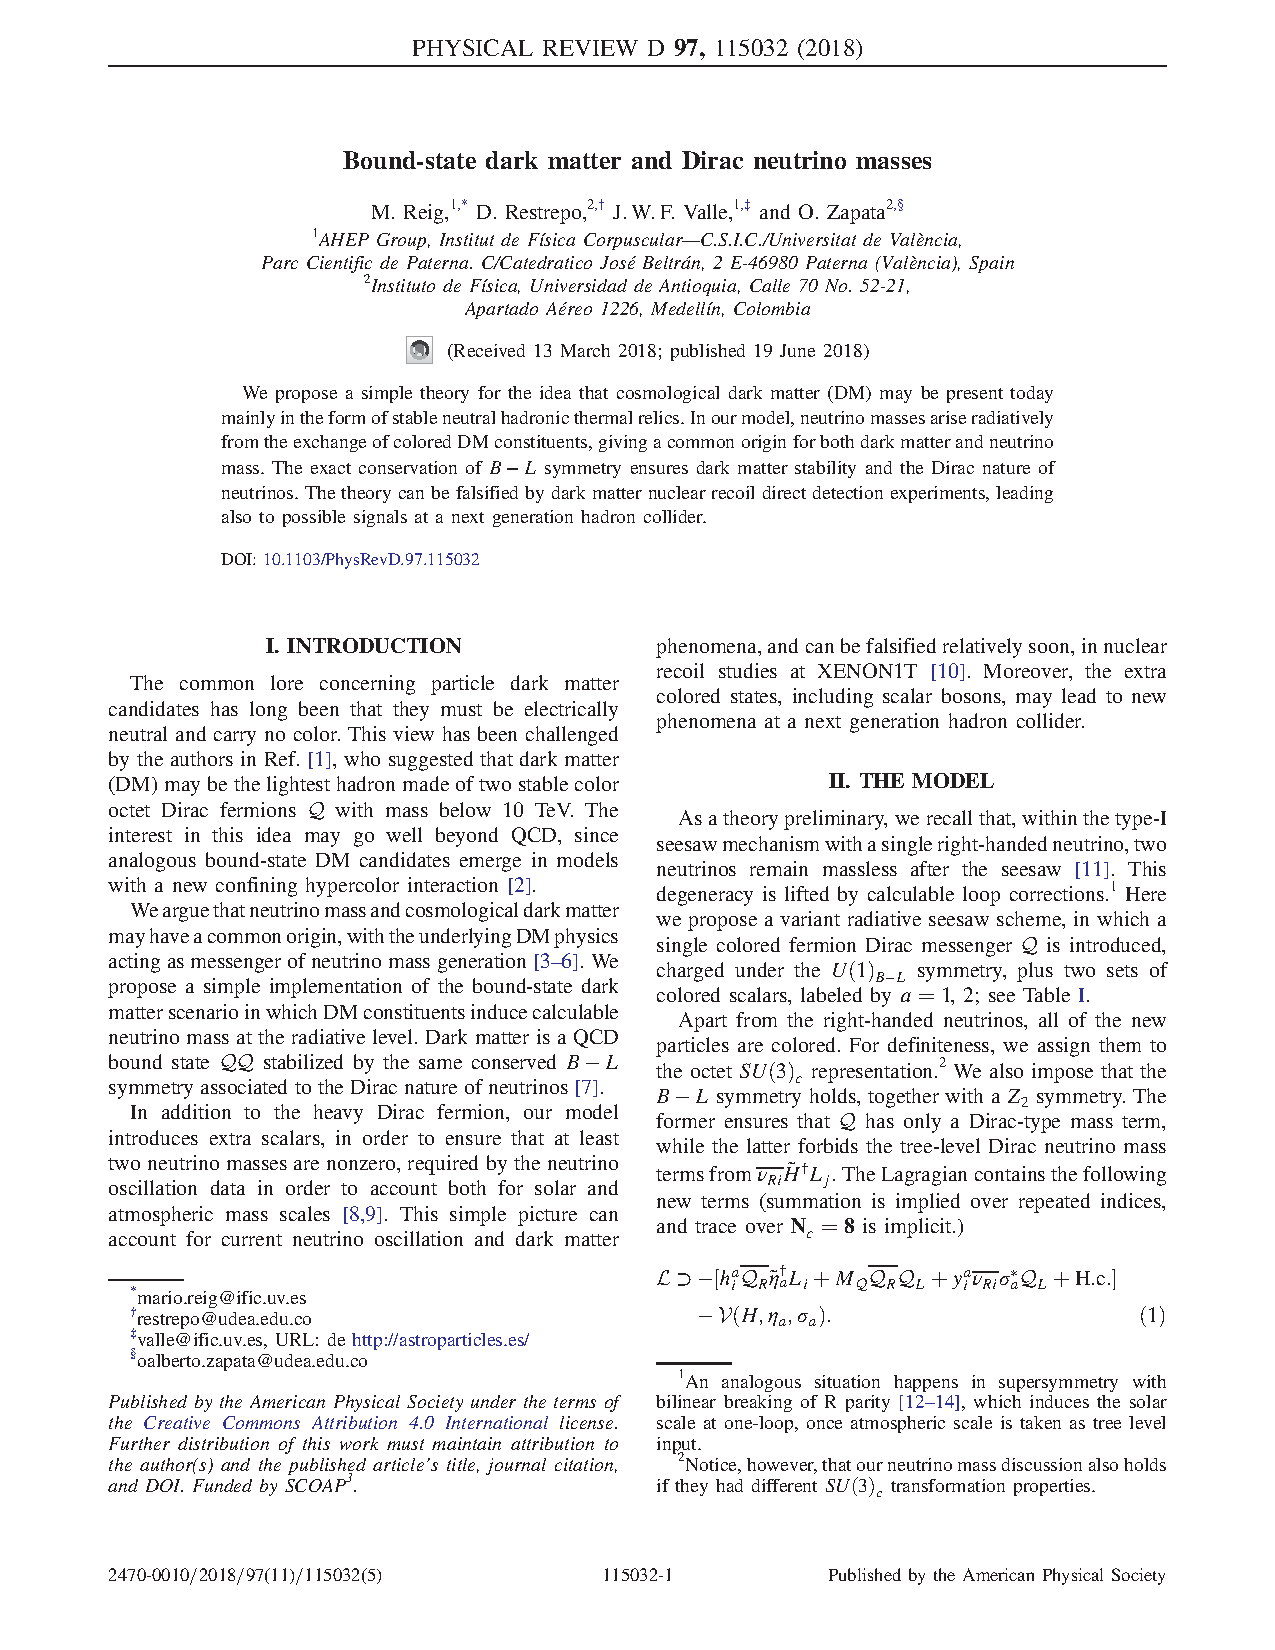
\includepdf[pages=-]{articles/PhysRevD-97-115032.pdf}  
%\end{includepdfs}

%\newpage{}


          


%%% Local Variables: 
%%% mode: latex
%%% TeX-master: "informefinal"
%%% ispell-local-dictionary: "castellano8"
%%% End: 

\end{document}

%%% Local Variables: 
%%% mode: latex
%%% TeX-master: "informefinal"
%%% End: 
